\chapter{Results} % Main appendix title
\label{Appendix-results} % For referencing this appendix elsewhere, use 
In this chapter we document results, based on the methodology used.

\section{CARLA Simulator results}
In this section we document simulation results, describing the code repository commit hash, and any relevant commands and outputs.
%%%%%%%%%%%%%%%%%%%%%%%%%%%%%%%%%%%%%%%%%%%%%%%%%%%%%%%%%%%%%%%%%%%%%%%%%%%%%
% RUN XXX - TEMPLATE - experiment log template
%%%%%%%%%%%%%%%%%%%%%%%%%%%%%%%%%%%%%%%%%%%%%%%%%%%%%%%%%%%%%%%%%%%%%%%%%%%%%
%\subsection{Run XXX -  }
%\label{app_res:XXX}
%\begin{verbatim}
%Commit:
%Model: 
%Outputs: 
%Dataset: 
%Command:
%Environment: 
%Comment: 
%\end{verbatim}

%%%%%%%%%%%%%%%%%%%%%%%%%%%%%%%%%%%%%%%%%%%%%%%%%%%%%%%%%%%%%%%%%%%%%%%%%%%%%
% RUN 001 - Running CARLA
%%%%%%%%%%%%%%%%%%%%%%%%%%%%%%%%%%%%%%%%%%%%%%%%%%%%%%%%%%%%%%%%%%%%%%%%%%%%%
\subsection{Run 001 - Running Carla}
\label{app_res:001}
\begin{verbatim}
Commit: bb4b95e0
Environment: Local desktop
Command:
$ make launch-only

Comment:
Simulator loads ok.

\end{verbatim}

%%%%%%%%%%%%%%%%%%%%%%%%%%%%%%%%%%%%%%%%%%%%%%%%%%%%%%%%%%%%%%%%%%%%%%%%%%%%%
% RUN 002 - Adding actors
%%%%%%%%%%%%%%%%%%%%%%%%%%%%%%%%%%%%%%%%%%%%%%%%%%%%%%%%%%%%%%%%%%%%%%%%%%%%%
\subsection{Run 002 - Adding actors}
\label{app_res:002}
\begin{verbatim}
Commit: bb4b95e0
Environment: Local desktop
Command:
$ make launch-only
# In another terminal, change directory to PythonAPI/examples, and run
$ python generate_traffic.py 
spawned 30 vehicles and 10 walkers, press Ctrl+C to exit.

Comment:
Simulator loads ok. The  default number of spawned vehicles is 30 and pedestrians (walkers) is 10. To change and other options, see script for details. The defaults in this case can be changed by adding switches:
$ python generate_traffic.py -n 60 -w 100
\end{verbatim}

\begin{figure}[h!]
\centering
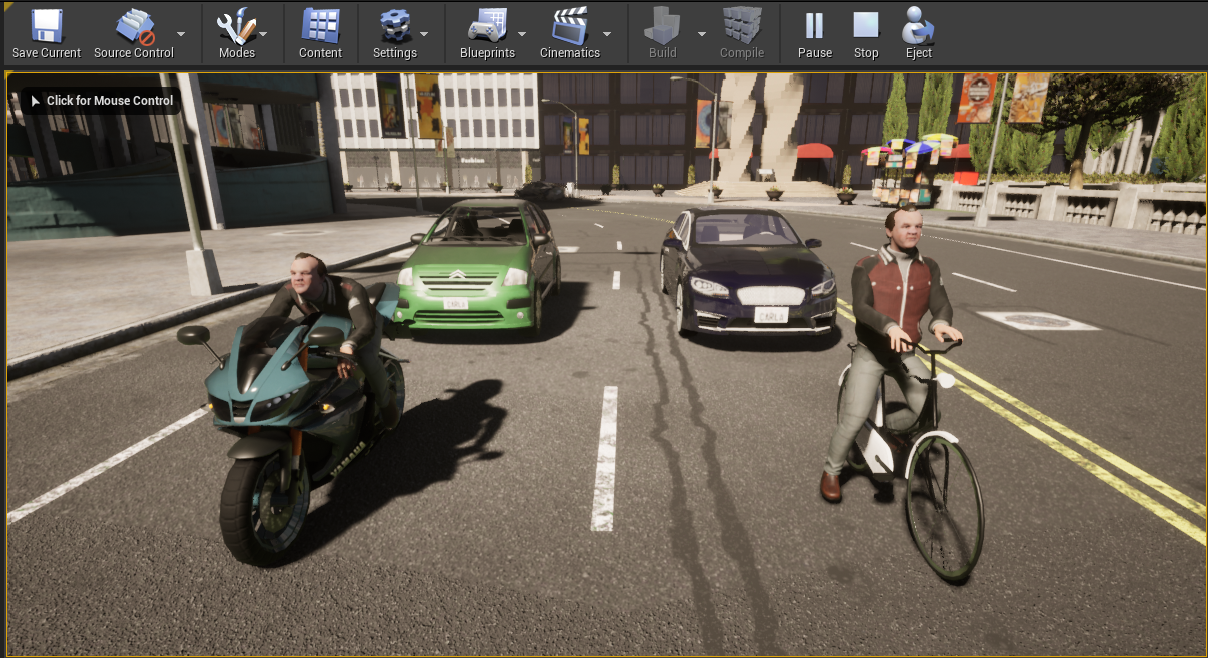
\includegraphics[width=\textwidth]{Figures/biker-cyclist.png}
\caption{CARLA simulator added actors}
\label{fig:biker-cyclist}
\end{figure}


%%%%%%%%%%%%%%%%%%%%%%%%%%%%%%%%%%%%%%%%%%%%%%%%%%%%%%%%%%%%%%%%%%%%%%%%%%%%%
% RUN 003 - Adding dynamic weather
%%%%%%%%%%%%%%%%%%%%%%%%%%%%%%%%%%%%%%%%%%%%%%%%%%%%%%%%%%%%%%%%%%%%%%%%%%%%%
\subsection{Run 003 - Adding dynamic weather}
\label{app_res:003}
\begin{verbatim}
Commit: bb4b95e0
Environment: Local desktop
Command:
$ make launch-only
# In another terminal, change directory to PythonAPI/examples, and run
$ python dynamic_weather.py -s 0.01
Sun(alt: -18.82, azm: 300.53) Storm(clouds=0%, rain=0%, wind=5%)            ^Z
[1]+  Stopped                 python3 dynamic_weather.py -s 0.01

Comment:
The parameter -s (speed) is a denominator in code, see
update_freq = 0.1 / speed_factor
The smaller the number, the less frequent (slower) are the weather updates, the greater the number, the more frequent (faster) are the weather updates.
\end{verbatim}

%%%%%%%%%%%%%%%%%%%%%%%%%%%%%%%%%%%%%%%%%%%%%%%%%%%%%%%%%%%%%%%%%%%%%%%%%%%%%
% RUN 004 - Automatic control
%%%%%%%%%%%%%%%%%%%%%%%%%%%%%%%%%%%%%%%%%%%%%%%%%%%%%%%%%%%%%%%%%%%%%%%%%%%%%
\subsection{Run 004 - Automatic control}
\label{app_res:004}
\begin{verbatim}
Commit: bb4b95e0
Environment: Local desktop
Date: 2021.11.21
Command:
$ make launch-only
# Once loaded, press play
# In another terminal, change directory to PythonAPI/examples, and run
$ python automatic_control.py

Comment:
This launches a pygame terminal, with a random vehicle set to ran
\end{verbatim}

%%%%%%%%%%%%%%%%%%%%%%%%%%%%%%%%%%%%%%%%%%%%%%%%%%%%%%%%%%%%%%%%%%%%%%%%%%%%%
% RUN 005 - Automatic control with traffic
%%%%%%%%%%%%%%%%%%%%%%%%%%%%%%%%%%%%%%%%%%%%%%%%%%%%%%%%%%%%%%%%%%%%%%%%%%%%%
\subsection{Run 005 - Automatic control with traffic}
\label{app_res:005}
\begin{verbatim}
Commit: bb4b95e0
Environment: Local desktop
Date: 2021.11.21
Command:
$ make launch-only
# Once loaded, press play
# In another terminal, change directory to PythonAPI/examples, and run
$ python generate_traffic.py 
spawned 30 vehicles and 10 walkers, press Ctrl+C to exit.

# In another terminal, change directory to PythonAPI/examples, and run
$ python automatic_control.py

Comment:
Traffic and automatic control vehicle are visible both in the pygame and unreal 
engine screens.
\end{verbatim}

%%%%%%%%%%%%%%%%%%%%%%%%%%%%%%%%%%%%%%%%%%%%%%%%%%%%%%%%%%%%%%%%%%%%%%%%%%%%%
% RUN 006 - Automatic control with traffic and dynamic weather
%%%%%%%%%%%%%%%%%%%%%%%%%%%%%%%%%%%%%%%%%%%%%%%%%%%%%%%%%%%%%%%%%%%%%%%%%%%%%
\subsection{Run 006- Automatic control with traffic and dynamic weather}
\label{app_res:006}
\begin{verbatim}
Commit: bb4b95e0
Environment: Local desktop
Date: 2021.11.21
Command:
$ make launch-only
# Once loaded, press play
# In another terminal, change directory to PythonAPI/examples, and run
$ python generate_traffic.py 
spawned 30 vehicles and 10 walkers, press Ctrl+C to exit.

# In another terminal, change directory to PythonAPI/examples, and run
$ python dynamic_weather.py -s 0.05
Sun(alt: -19.78, azm: 300.10) Storm(clouds=0%, rain=0%, wind=5%)  

# In another terminal, change directory to PythonAPI/examples, and run
$ python automatic_control.py

Comment:
The sun position changes every two seconds when parameter -s 0.05 is 
passed (0.1 / 0.05 = 2)

To exit the simulation:
1. Ensure dynamic_weather.py is not running or stop with CONTROL + C
2. Stop generate_traffic.py with CONTROL + C
3. Stop dynamic_weather.py with CONTROL + C
4. Stop Unreal Engine

If script generate_traffic.py is not stopped with CONTROL + C, and say CONTROL + Z, may still be running in the background. This will keep a lock on the port.

To list processes (open files) that have port 2000 open:
$ sudo lsof -t -i:2000
3281
3416

To check which process the process ID listed refers to:
$ ps aux | grep 3281
daniel    3281  0.9  0.2 1860476 90348 pts/1   Tl   17:25   0:29 python3 generate_traffic.py
daniel    7455  0.0  0.0  14432  1040 pts/1    S+   18:18   0:00 grep --color=auto 3281

To kill the process:
$ sudo kill -9 3281
[1]+  Killed                  python3 generate_traffic.py

\end{verbatim}

\begin{figure}[h!]
\centering
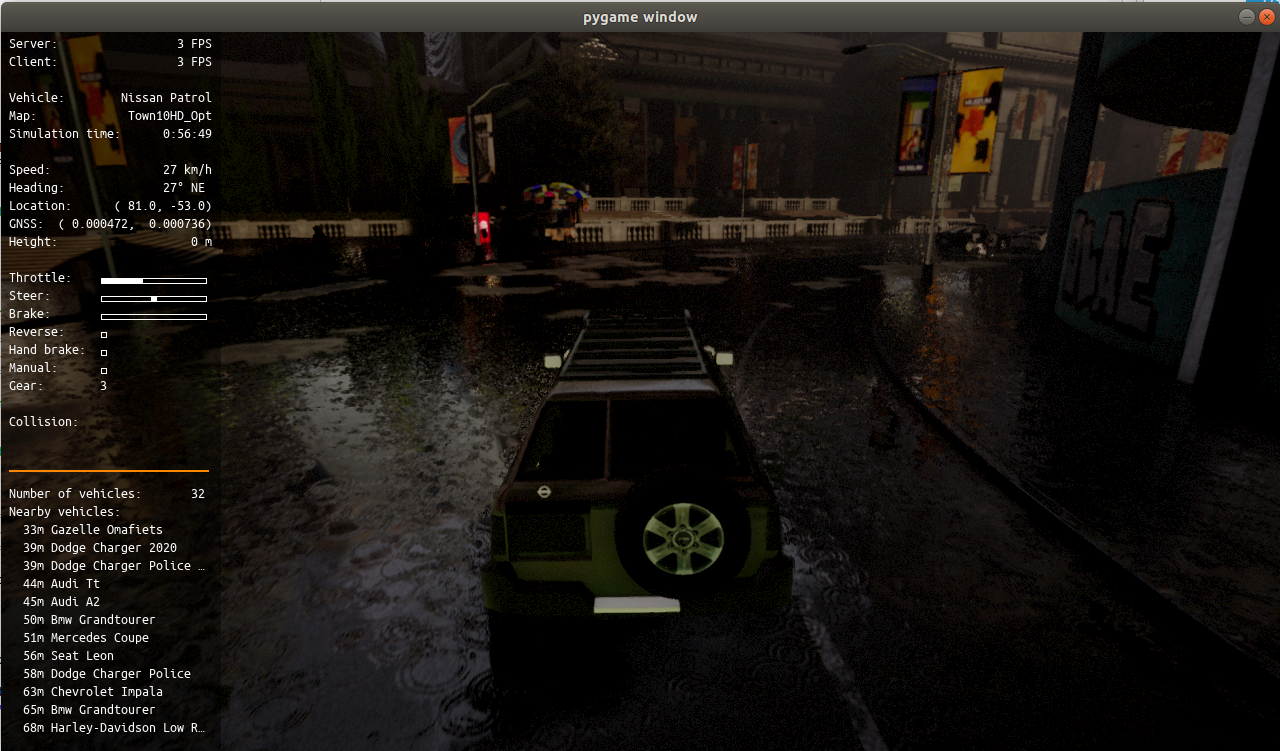
\includegraphics[width=\textwidth]{Figures/carla-rain.png}
\caption{CARLA simulator with dynamic weather}
\label{fig:carla-rain}
\end{figure}

\begin{figure}[h!]
\centering
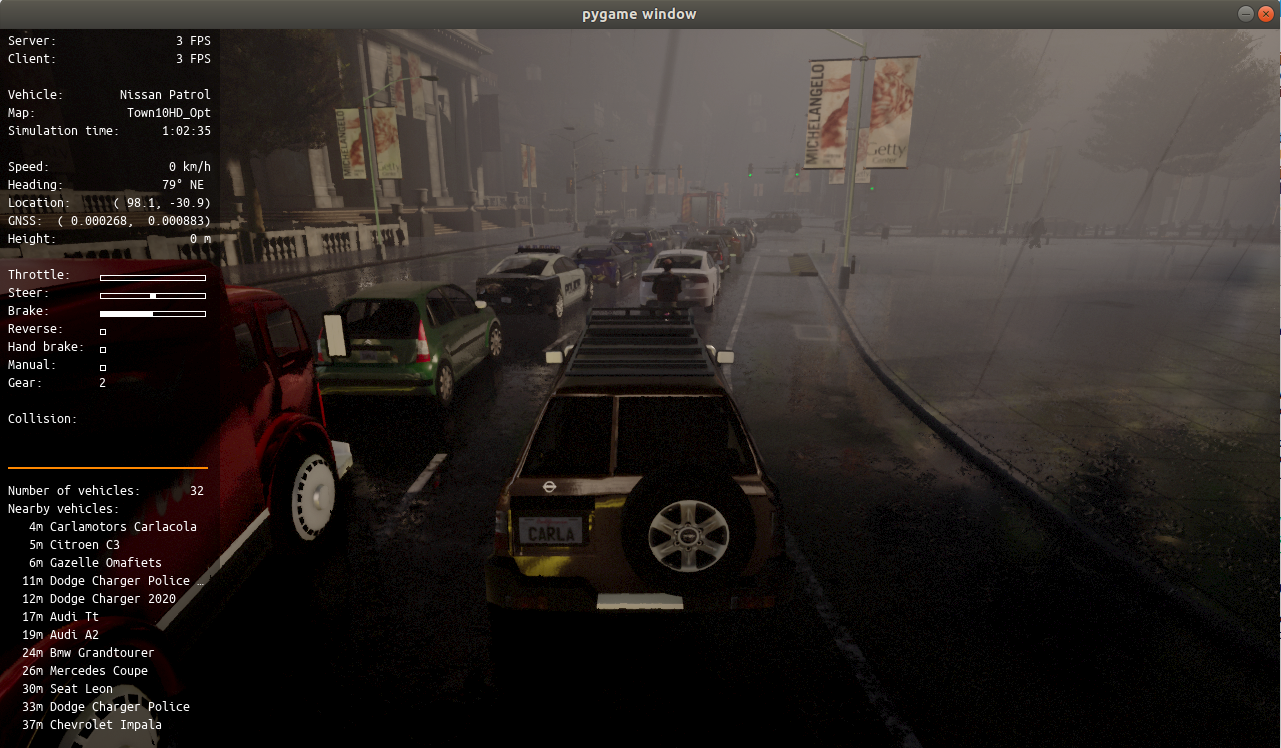
\includegraphics[width=\textwidth]{Figures/carla-traffic-jam.png}
\caption{CARLA simulator traffic jam}
\label{fig:carla-traffic-jam}
\end{figure}

Figures \ref{fig:carla-rain} and \ref{fig:carla-traffic-jam} are taken from the pygame screen.

\begin{figure}[h!]
\centering
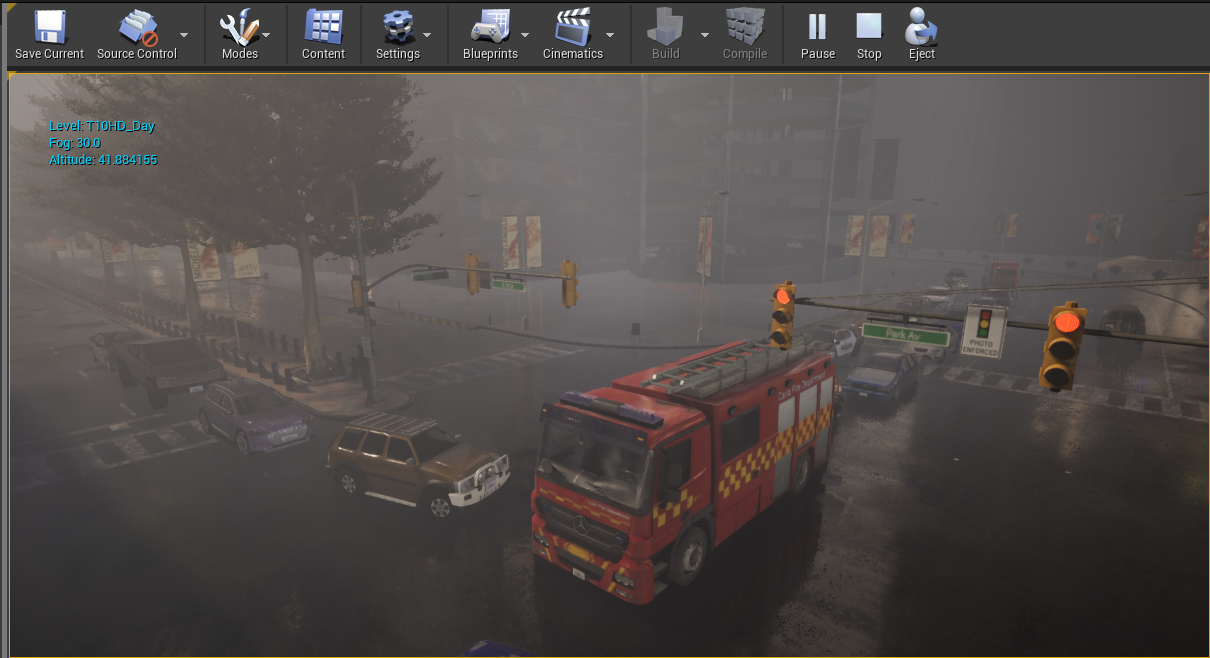
\includegraphics[width=\textwidth]{Figures/carla-traffic-jam-2.png}
\caption{CARLA simulator traffic jam reverse angle}
\label{fig:carla-traffic-jam-2}
\end{figure}

Figure \ref{fig:carla-traffic-jam-2}, taken from Unreal Engine, showing the stopped vehicles at the T-junction and is the reverse angle of Figure \ref{fig:carla-traffic-jam}. note there has not been a collision. The algorithm driving each vehicle seems to be stuck by a proximity assessment that is unlikely to change given all vehicles are stopped.

%%%%%%%%%%%%%%%%%%%%%%%%%%%%%%%%%%%%%%%%%%%%%%%%%%%%%%%%%%%%%%%%%%%%%%%%%%%%%
% RUN 007 - Automatic control with traffic
%%%%%%%%%%%%%%%%%%%%%%%%%%%%%%%%%%%%%%%%%%%%%%%%%%%%%%%%%%%%%%%%%%%%%%%%%%%%%
\subsection{Run 007- Automatic control with traffic}
\label{app_res:007}
\begin{verbatim}
Commit: bb4b95e0
Environment: Local desktop
Date: 2021.11.22
Commands:
$ make launch-only
# Loaded Town04_Opt
$ python generate_traffic.py -n 60 -w 600
spawned 60 vehicles and 328 walkers, press Ctrl+C to exit.
# NB some walkers not created due to collisions
# In another terminal, change directory to PythonAPI/examples, and run
$ python automatic_control.py

Comment:
Various successive runs, number of vehicles decreasing over time due to collisions. One simulated self-drving vehicle got stuck in the simulation (tipycally it would be destroyed at the end of self-driving simulation) after crashing against a traffic-light post.
\end{verbatim}

%%%%%%%%%%%%%%%%%%%%%%%%%%%%%%%%%%%%%%%%%%%%%%%%%%%%%%%%%%%%%%%%%%%%%%%%%%%%%
% RUN 008 - Using the same vehicle
%%%%%%%%%%%%%%%%%%%%%%%%%%%%%%%%%%%%%%%%%%%%%%%%%%%%%%%%%%%%%%%%%%%%%%%%%%%%%
\subsection{Run 008 - Using the same vehicle}
\label{app_res:008}
\begin{verbatim}
Commit: bb4b95e0
Environment: Local desktop
Date: 2021.12.05
Commands:
$ make launch-only
# Loaded Town10HD_Opt (current default)
# pressed "Play"
# generated dynamic weather
$ python dynamic_weather.py --speed 0.1
# generate traffic
$ python generate_traffic.py -n 60 -w 600
(...)
Vehicle agent not added to the crowd by some problem!
(...)
# error message assumed to caused by starting sequence i.e. dynamic weather before dynamic traffic.
$ python generate_traffic.py -n 60 -w 600

Comment:
Currently code uses a random vehicle chosen in automatic_control.py. All cars vanished from simulation two hours in. Pedestrians still present.
\end{verbatim}


%%%%%%%%%%%%%%%%%%%%%%%%%%%%%%%%%%%%%%%%%%%%%%%%%%%%%%%%%%%%%%%%%%%%%%%%%%%%%
% RUN 009 - Hyperion test
%%%%%%%%%%%%%%%%%%%%%%%%%%%%%%%%%%%%%%%%%%%%%%%%%%%%%%%%%%%%%%%%%%%%%%%%%%%%%
\subsection{Run 009 - Hyperion High Computing Cluster Test}
\label{app_res:009}
\begin{verbatim}
Repository: https://github.com/dsikar/mscai
Branch: master
Commit: d4409a20
Environment: Hyperion
Date: 2022.03.20
Connection details:
As per "HPC - How to connect using windows"
Commands:
$ cd ~/localscratch 
$ git clone https://github.com/dsikar/mscai
$ cd Lab1
# deactivate environment - activated by default in ~/.bashrc
$ flight env deactivate
# run
$ source /opt/flight/etc/setup.sh
$ flight env activate singularity
$ singularity exec --nv /mnt/scratch/singularity/psarin/ubuntu20_04cuda11.sif \  /usr/bin/python3 /users/aczd097/localscratch/mscai/Lab1/DLIALab1.py

Comment:
This script is supposed to run with 
aczd097@login1 ~/localscratch/mscai/Lab1 (master)$ sbatch runModel.sh
Submitted batch job 173522

The JOBID does not appear in the queue. Assumption is job fails to start.

from: https://sylabs.io/guides/3.7/user-guide/definition_files.html
The process of creating the singularity container (.sif file) is:

1. A script is created:
/mnt/scratch/singularity/psarin/ubuntu20_04cuda11.def
2. And built:
$ sudo singularity build --notest my_container.sif my_container.def

\end{verbatim}


%%%%%%%%%%%%%%%%%%%%%%%%%%%%%%%%%%%%%%%%%%%%%%%%%%%%%%%%%%%%%%%%%%%%%%%%%%%%%
% RUN XXX - Template
%%%%%%%%%%%%%%%%%%%%%%%%%%%%%%%%%%%%%%%%%%%%%%%%%%%%%%%%%%%%%%%%%%%%%%%%%%%%%
\subsection{Run XXX - Template}
\label{app_res:XXX}
\begin{verbatim}
Commit: bb4b95e0
Environment: Local desktop
Date: 2021.12.05
Commands:
$ make launch-only
# Loaded Town10HD_Opt (current default)
# pressed "Play"
# generated dynamic weather
$ python dynamic_weather.py --speed 0.1
# generate traffic
$ python generate_traffic.py -n 60 -w 600
(...)
Vehicle agent not added to the crowd by some problem!
(...)
# error message assumed to caused by starting sequence i.e. dynamic weather before dynamic traffic.
$ python generate_traffic.py -n 60 -w 600

Comment:
Currently code uses a random vehicle chosen in automatic_control.py. All cars vanished from simulation two hours in. Pedestrians still present.
\end{verbatim}
